\documentclass[stu, 12pt, letterpaper, donotrepeattitle, floatsintext, natbib]{apa7}
\usepackage[utf8]{inputenc}
\usepackage{graphicx}
\usepackage{float} %\begin{}[H]
\usepackage[spanish]{babel} 

% 
\usepackage{amsmath}
\usepackage{xcolor}
\usepackage{cancel}
\usepackage{paracol}

\selectlanguage{spanish}
\newcommand{\myparagraph}[1]{\paragraph{#1}\mbox{}\\}

% Portada
\thispagestyle{empty}
\title{\Large Calculo Diferencial e Integral}
\author{Cristian Herrera}
\affiliation{Instituto Superior Tecnológico Tena}
\course{Calculo Diferencial e Integral}
\professor{Ing. Libinton Lara}
\duedate{2023 - IIP}


\begin{document}
\maketitle

% Índices
\pagenumbering{roman}
    % Contenido
\renewcommand\contentsname{\largeÍndice}
\tableofcontents
\setcounter{tocdepth}{6} % ALCANCE DEL INDICE
\newpage
    % Fíguras
% \renewcommand{\listfigurename}{\largeÍndice de fíguras}
% \listoffigures
% \newpage
    % Tablas
% \renewcommand{\listtablename}{\largeÍndice de tablas}
% \listoftables
% \newpage

% Cuerpo
\pagenumbering{arabic}

\section{Actividades en Clase}
\subsection{Matrices y Determinantes} 

\subsubsection{Que es una matriz?}
Conjunto bidimencional de numeros o simbolos que sirven para describir y resolver sistemas de ecuaciones lineales.
\begin{table}
    \centering
    \begin{tabular}{|c|c|}
        \hline
        Sistema de Ecuaciones & En Forma de Matriz \\ \hline
        & $\quad x\quad y\quad i$ \\ 
        $ f(x) =  \begin{cases} x + 3y = 7 \\ 5x - y = 3  \end{cases} $ 
        & 
        $A = \begin{pmatrix}
            1 & 3 & 7 \\
            5 & -1 & 3
        \end{pmatrix}_{2\times3}$ \\[1cm]\hline
        
        & $\quad\quad\quad x\quad i\quad $ \\
        $2x=4$ & $A = \begin{pmatrix} 2 & 4 \end{pmatrix}$ \\[0.8cm]\hline
        
        & $\quad\quad x\quad\quad y\quad\quad z\quad\quad i$ \\
        $ f(x)=\begin{cases} 3x-5y+8z=10 \\ 2y-7z=-15 \end{cases} $ & 
        $C=\begin{pmatrix}
            3 & -5 & 8 & 10 \\ 
            0 & 2 & -2 & -15
        \end{pmatrix}$ \\[1cm]\hline
    \end{tabular}
\end{table}

\subsubsection{Dimensiones de una matriz}
$$
A=\begin{pmatrix}
a_{11} & a_{12} & a_{13} & a_{14}\\
a_{21} & a_{22} & a_{23} & a_{24}\\
\end{pmatrix}_{M\times N}
$$\\
\begin{small}
\begin{center}
$M= $Filas, $N= $Columnas
\end{center}
\end{small}

Un elemento de una matriz se representa: {\Large $a_{ij}$}, donde {\Large $i$} representa las filas, y {\Large $j$} las columnas\\

\subsubsection{Tipos de Matrices}
\paragraph{Matriz Fila (Vector Fila)}
Matriz formada por una sola fila.
$$A=\begin{pmatrix} a_{11} & a_{12} & a_{13} & .... & a_{1n} \end{pmatrix}_{1\times n}$$
\paragraph{Matriz Columna (Vector Columna)}
Matriz formada por una sola columna.
$$A=\begin{pmatrix} a_{11} \\ a_{21} \\ a_{31} \\ ... \\ ... \\ ... \\ a_{m1}\end{pmatrix}_{m\times1}$$
\paragraph{Matriz Nula}
Todos sus elementos son nulos
$$A=\begin{pmatrix} 0 & 0 & 0 & 0 \\ 0 & 0 & 0 & 0 \end{pmatrix}_{2\times4}$$
\paragraph{Matriz Cuadrada}
Tiene el mismo numero de filas y de columnas.

\begin{table}
\centering
\begin{tabular}{cc}
$
A = \begin{pmatrix}
    \color{red} a_{11} & a_{12} & a_{13} \\
    a_{21} & \color{red} a_{22} & a_{23} \\
    a_{31} & a_{32} & \color{red} a_{33} \\
\end{pmatrix}_{3\times3}
$
&
$
B = \begin{pmatrix}
    a_{11} & a_{12} & \color{blue} a_{13} \\
    a_{21} & \color{blue} a_{22} & a_{23} \\
    \color{blue} a_{31} & a_{32} & a_{33} \\
\end{pmatrix}_{3\times3}
$
\end{tabular}
\end{table}
\subparagraph{Elementos básicos de una Matriz Cuadrada}
\myparagraph{Diagonal Mayor}
Formada por los elementos $\color{red} a_{11}$, $\color{red} a_{22}$, $\color{red} a_{33}$, $\color{red} \ldots$, $\color{red} a_{nn}$.
\myparagraph{Diagonal Menor}
Formada por los elementos {\Large $\color{blue} a_{ij}$} donde {\normalsize $\color{blue} i+j = n+1$}
\myparagraph{Traza}
Suma de los elementos de la diagonal principal.

\begin{table}
\centering
\begin{tabular}{cc}
$
A=\begin{pmatrix}
\color{red} -2 & 6 & 4 \\
8 & \color{red} 12 & -9 \\
15 & -6 & \color{red} -4
\end{pmatrix}
$ & traza: $-2 +12 -4 = 6$
\end{tabular}
\end{table}

\subparagraph{Tipos básicos de matrices cuadradas}
\myparagraph{Triangular Superior}
Todos los elementos son ceros debajo de la diagonal principal.
$$
A=\begin{pmatrix}
\color{gray} -2 & \color{gray} 6 & \color{gray} 4 \\
0 & \color{gray} 12 & \color{gray} -9 \\
0 & 0 & \color{gray} -4
\end{pmatrix}
$$
\myparagraph{Triangular Inferior}
Encima de la diagonal principal todos son ceros.
$$
A=\begin{pmatrix}
\color{gray} -2 & 0 & 0 \\
\color{gray} 8 & \color{gray} 12 & 0 \\
\color{gray} 15 & \color{gray} -6 & \color{gray} -4
\end{pmatrix}
$$
\myparagraph{Matriz Diagonal}
Los elementos que no están en la diagonal principal son ceros, esta también es una matriz triangular superior y triangular inferior.
$$
A=\begin{pmatrix}
\color{gray} -2 & \textbf{0} & \textbf{0} \\
\textbf{0} & \color{gray} 12 & \textbf{0} \\
\textbf{0} & \textbf{0} & \color{gray} -4
\end{pmatrix}
$$
\myparagraph{Matriz identidad o unidad}
Es una matriz diagonal, en la que todos los elementos de la diagonal principal son 1.
\[
A=\begin{bmatrix}
\textbf{1} & 0 & 0 \\ 
0 & \textbf{1} & 0 \\
0 & 0 & \textbf{1}
\end{bmatrix}
\]
\myparagraph{Matriz Escalar}
Es una matriz diagonal, en la que todos los elementos de la diagonal principal son iguales.
\[
A=\begin{bmatrix}
\textbf{5} & \color{gray} 0 & \color{gray} 0 \\ 
 \color{gray} 0 & \textbf{5} & \color{gray} 0 \\
 \color{gray}0 &  \color{gray} 0 & \textbf{5}
\end{bmatrix}
\]
\subsubsection{Suma de Matrices}
Se puede dar entre matrices del mismo orden, para realizar la suma se debe sumar cada elemento de una posición con otro elemento de una matriz de la misma posición.

\begin{table}
\centering
\begin{tabular}{c}
$
A=\begin{pmatrix}
a_{11} & a_{12} & a_{13} & a_{14}\\
a_{21} & a_{22} & a_{23} & a_{24}\\
\end{pmatrix}_{2\times4}
$  $
B=\begin{pmatrix}
b_{11} & b_{12} & b_{13} & b_{14}\\
b_{21} & b_{22} & b_{23} & b_{24}\\
\end{pmatrix}_{2\times4}
$\\ \\ $
A+B=\begin{pmatrix}
(a_{11} + b_{11})_{11} & (a_{12} + b_{12})_{12} & (a_{13} + b_{13})_{13} & (a_{14} + b_{14})_{14}\\
(a_{21} + b_{21})_{21} & (a_{22} + b_{22})_{22} & (a_{23} + b_{23})_{23} & (a_{24} + b_{24})_{24}\\
\end{pmatrix}_{2\times4}
$

\end{tabular}
\end{table}

\subsubsection{Resta de Matrices}
Se puede dar entre matrices del mismo orden, para realizar la resta se debe restar cada elemento de una posición con otro elemento de una matriz de la misma posición.

\begin{table}[H]
\centering
\begin{tabular}{c}
$
A=\begin{pmatrix}
a_{11} & a_{12} & a_{13} & a_{14}\\
a_{21} & a_{22} & a_{23} & a_{24}\\
\end{pmatrix}_{2\times4}
$  $
B=\begin{pmatrix}
b_{11} & b_{12} & b_{13} & b_{14}\\
b_{21} & b_{22} & b_{23} & b_{24}\\
\end{pmatrix}_{2\times4}
$\\ \\ $
A-B=\begin{pmatrix}
(a_{11} - b_{11})_{11} & (a_{12} - b_{12})_{12} & (a_{13} - b_{13})_{13} & (a_{14} - b_{14})_{14}\\
(a_{21} - b_{21})_{21} & (a_{22} - b_{22})_{22} & (a_{23} - b_{23})_{23} & (a_{24} - b_{24})_{24}\\
\end{pmatrix}_{2\times4}
$

\end{tabular}
\end{table}

\newpage

\subsubsection{Producto De Una Matriz Por Un Escalar/Real}
La multiplicación de una matriz por un escalar se realiza multiplicando el escalar por cada elemento de la matriz.

\begin{table}[H]
\centering
\begin{tabular}{ccc}
$
\dfrac{3}{2} \times \begin{pmatrix}
2 & -4\\
1 & -8\\
\end{pmatrix}_{2\times2}
$  & $=$ & $
\begin{pmatrix}
3 & -6 \\
\frac{3}{2} & -12\\
\end{pmatrix}_{2\times2}
$\\ 

\end{tabular}
\end{table}


\subsubsection{Multiplicación de Matrices}
Es posible si el numero de \textbf{columnas} de la primera matriz es el mismo al numero de \textbf{filas} de la segunda matriz.
Para multiplicar dos matrices cuadradas, calcula el producto de filas de la primera matriz con columnas de la segunda matriz y suma los resultados.
$$
A=\begin{pmatrix}
1 & 3 \\ 4 & 5
\end{pmatrix}_{2\times2}
\qquad
B=\begin{pmatrix}
6 & 7 \\ 8 & 9
\end{pmatrix}_{2\times2}
$$\\

¿Es posible multiplicar la matriz A por la matriz B?
$${\textit{2}\times\textbf{2}} \qquad {\textbf{2}\times\textit{2}}$$\\

Si es posible ya que el numero de columnas de la primera fila es el mismo que el numero de filas de la segunda, $\textbf{2}$ = $\textbf{2}$, ademas el resultado de $A\times B$ sera igual a una matriz de $\textit{2} \times \textit{2}$.
\begin{center}
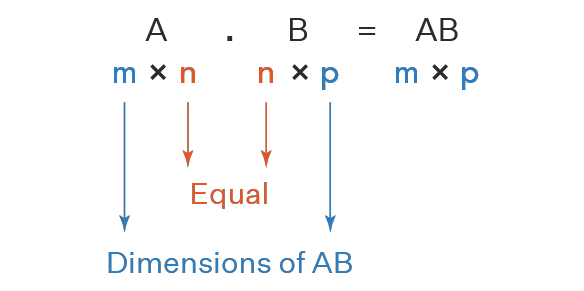
\includegraphics[scale=0.5]{matrix.png} \\
\[
\begin{bmatrix}
   \color{blue} 2 & \color{blue} 3 \\
    \color{red} 4 & \color{red} 5
\end{bmatrix}
\times
\begin{bmatrix}
    \color{green} 6 & \color{violet} 7 \\
    \color{green} 8 & \color{violet} 9
\end{bmatrix}
=
\begin{bmatrix}
    (\color{blue} 2 \textcolor{black}{\,\cdot\,} \color{green} 6 \textcolor{black}{\,+\,} \color{blue} 3 \textcolor{black}{\,\cdot\,} \textcolor{green}{8} \textcolor{black}{)} 
    &
     (\color{blue} 2 \textcolor{black}{\,\cdot\,} \color{violet} 7 \textcolor{black}{\,+\,} \color{blue} 3 \textcolor{black}{\,\cdot\,} \textcolor{violet}{9} \textcolor{black}{)} \\
          
    (\color{red} 4 \textcolor{black}{\,\cdot\,} \color{green} 6 \textcolor{black}{\,+\,} \color{red} 5 \textcolor{black}{\,\cdot\,} \textcolor{green}{8} \textcolor{black}{)}
    &    
    (\color{red} 4 \textcolor{black}{\,\cdot\,} \color{violet} 7 \textcolor{black}{\,+\,} \color{red} 5 \textcolor{black}{\,\cdot\,} \textcolor{violet}{9} \textcolor{black}{)}
\end{bmatrix}
= AB=
\begin{bmatrix}
    36 & 41 \\
    68 & 77
\end{bmatrix}_{2\times2}
\]
\end{center}


\subsubsection{Determinantes}
El determinante de una matriz solo existe en matrices cuadradas.
\paragraph{Determinante 2x2}
Se calcula restando el producto de los números que conforman la diagonal secundaria al producto de los números que conforman la diagonal principal. 
\[
A=\begin{pmatrix}
b & c \\ d & e
\end{pmatrix}
\qquad
\qquad
|A|= (be) - (cd)
\]
\paragraph{Determinante 3x3 - Regla de Sarrus}
Las primeras columnas o columnas de la matriz se repiten al final y se realiza una multiplicación de diagonales para obtener el determinante.\\
\begin{table}
\begin{tabular}{cc}

Primera forma & Segunda forma \\
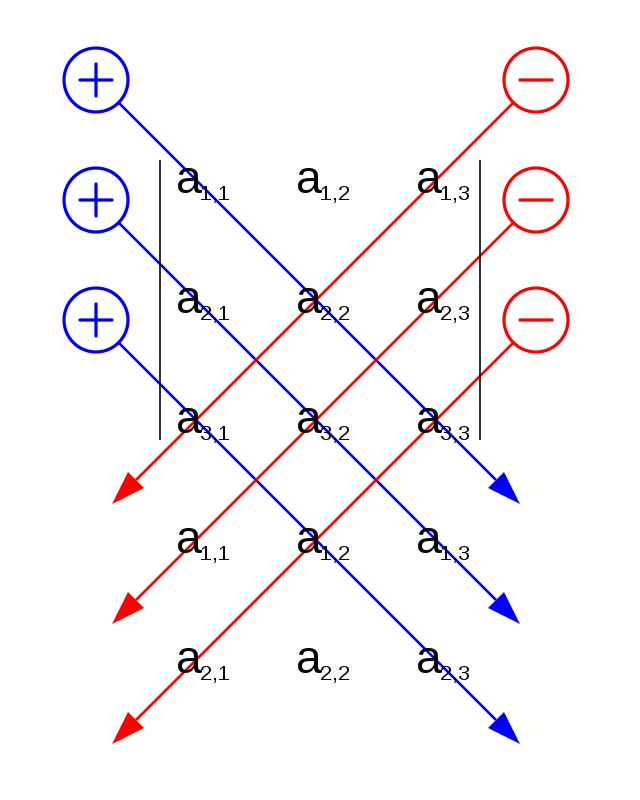
\includegraphics[scale=0.25]{sarrus}
&
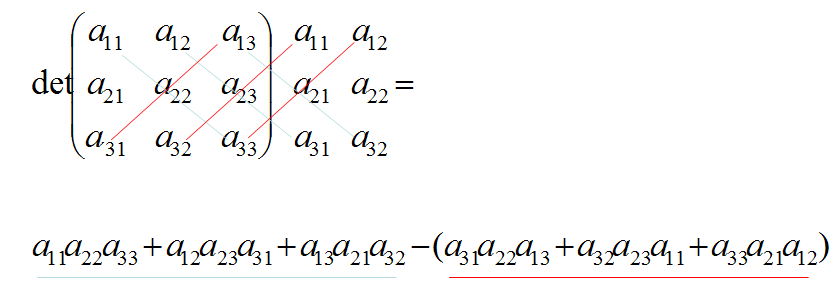
\includegraphics[scale=0.5]{sarrus2}

\end{tabular}
\end{table}

\subsubsection{Matriz Transpuesta}
La matriz traspuesta de una matriz se denota por y se obtiene cambiando sus filas por columnas (o viceversa).
\[
Z =
\begin{pmatrix}
\color{red} a &\color{red} b & \color{red}c \\
\color{blue} d & \color{blue}e & \color{blue}f 
\end{pmatrix}
\qquad \qquad
Z^T =
\begin{pmatrix}
\color{red}a & \color{blue}d \\ 
\color{red}b & \color{blue}e \\
\color{red}c & \color{blue}f \\
\end{pmatrix}
\]

\subsubsection{Igualdad de Matrices}
\begin{itemize}
\item \begin{equation*}
\begin{pmatrix}
 a & b \\
 c & d 
\end{pmatrix}
\quad
+
\quad
\begin{pmatrix}
 1 & 3 \\
 2 & 4 
\end{pmatrix}
\quad
=
\quad
\begin{pmatrix}
0 & 2 \\
1 & 3
\end{pmatrix}
\end{equation*}

\begin{equation*}
\begin{pmatrix}
a+1 & b+3 \\
c+2 & d+4
\end{pmatrix}_{2\times 2}
\quad
=
\quad
\begin{pmatrix}
0 & 2 \\
1 & 3
\end{pmatrix}
\end{equation*}

\begin{table}
\centering
\begin{tabular}{ccc}
$a+1=0$ & $\qquad$ & $b+3=2$ \\
$a=-1$ & & $b=-1$ \\
\\
$c+2=1$ & & $d+4=3$ \\
$c=-1$ & & $d=-1$
\end{tabular}
\end{table}


\item \begin{equation*}
\begin{pmatrix}
0 & x \\
2 & -1
\end{pmatrix}
=
\begin{pmatrix}
0 & 2 \\
2 & -1
\end{pmatrix}
\end{equation*}
\begin{center}
Cumple si $x=2$
\end{center}
\end{itemize}

\subsubsection{Producto de un Escalar por un Determinante}
Se multiplica el numero escalar por toda una fila o columna, a continuación se muestra un ejemplo en el cual seleccione la primera columna.

\[
2 \cdot
\begin{vmatrix}
  \color{red}1 & \color{red}4 & \color{red}2 \\
  1 & 5 & 2 \\
  2 & -1 & 0 \\
\end{vmatrix}
=
\begin{vmatrix}
  2 & 8 & 4 \\
  1 & 5 & 2 \\
  2 & -1 & 0
\end{vmatrix}
\]
\newpage
\subsubsection{Matriz Adjunta}
${Adj}(A)={C_A}^T$	\qquad \qquad \qquad -->	$C_{ij}=(-1)^{i+j} |A_{ij}|$
\begin{itemize}

\item $2 \times 2$ \\[0.5cm]
\begin{tabular}{ccc}
$A= \begin{pmatrix} 1 & 2 \\ -4 & 5 \end{pmatrix}$ \quad &
$C_A= \begin{pmatrix} +(5) & -(-4) \\ -(2) & +(1) \end{pmatrix}$ \quad &
${C_A}^T = {Adj}(A)=\begin{pmatrix} 5 & -2 \\ 4 & 1 \end{pmatrix}$
\end{tabular} \\[1cm]

\item $3 \times 3$ \\[0.5cm]
\begin{table}
\centering
\begin{tabular}{ccc}
$B= \begin{pmatrix} 
2 & -1 & 0 \\
3 & 6 & 1 \\
4 & 0 & 2
\end{pmatrix}$ \quad &
$C_B= \begin{pmatrix} 
+(12) & -(2) & +(-24) \\
-(-2) & +(4) & -(4) \\
+(-1) & -(2) & +(15) \end{pmatrix}$ \quad &
${C_B}^T = {Adj}(B)=\begin{pmatrix} 
12 & 2 & -1 \\
-2 & 4 & -2 \\
-24 & -4 & 15 \end{pmatrix}$
\end{tabular}
\end{table}
\end{itemize}

\subsubsection{Menor de una Matriz}
En el siguiente ejemplo vemos el menor de $A_{11}$ ($M_{ij}$) señalado con azul.
$$A=\begin{pmatrix}
\color{red}1 &  \cancel{3} & \cancel{4} \\
\cancel{-1} & \color{blue}2 & \color{blue}-1 \\
\cancel{3} & \color{blue}2 & \color{blue}-5
\end{pmatrix} 	\qquad \qquad \qquad	M_{ij}$$

$M_{11}=\left| \begin{matrix}
2 & -1 \\ 2 & -5 \end{matrix} \right| = -8$
\qquad
$M_{12}=\left| \begin{matrix}
-1 & -1 \\ 3 & -5 \end{matrix} \right| = 8$
\qquad
$M_{13}=\left| \begin{matrix}
-1 & 2 \\ 3 & 2 \end{matrix} \right| = -8$ \\[0.4cm]


$M_{21}=\left| \begin{matrix}
3 & 4 \\ 2 & -5 \end{matrix} \right| = -23$
\qquad
$M_{22}=\left| \begin{matrix}
1 & 4 \\ 3 & -5 \end{matrix} \right| = -17$
\qquad
$M_{23}=\left| \begin{matrix}
1 & 3 \\ 3 & 2 \end{matrix} \right| = -7$\\[0.4cm]


$M_{31}=\left| \begin{matrix}
3 & 4 \\ 2 & -1 \end{matrix} \right| = -11$
\qquad
$M_{32}=\left| \begin{matrix}
1 & 4 \\ -1 & -1 \end{matrix} \right| = 3$
\qquad
$M_{33}=\left| \begin{matrix}
1 & 3 \\ -1 & 2 \end{matrix} \right| = 5$ \\

\newpage
\paragraph{Cofactor} $C_{ij}
=(-1)^{i+j}M_{ij}$ \\
\begin{table}[H]
\begin{tabular}{c}
$C_{21}=(-1)^{2+1}M_{21}$ \\
$C_{21}=(-1)^3(-23)$ \\
$C_{21}=23$
\end{tabular}
\hspace{5cm}
\begin{tabular}{c}
$C_A=\begin{pmatrix}
C_{11} & C_{12} & C_{13} \\
C_{21} & C_{22} & C_{23} \\
C_{31} & C_{32} & C_{33} \\
\end{pmatrix}
=
\begin{pmatrix}
-8 & -8 & -8 \\
23 & 17 & 7 \\
-11 & -3 & 5
\end{pmatrix}
$
\end{tabular} \\
\end{table}

\subsubsection{Calculo del determinante por Cofactores}
El determinante por el método de cofactores, es el resultado de la suma de los productos de cada elemento multiplicado por su cofactor de toda una fila o toda una columna\\
\begin{center}
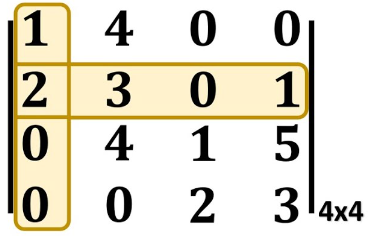
\includegraphics[scale=0.5]{dc.png}
\end{center}

\begin{itemize}
\item $
A= \begin{pmatrix}
1 & 3 & 4 \\ -1 & 2 & -1 \\ 3 & 2 & -5
\end{pmatrix}
$
\vspace{0.5cm}
En este caso he escogido la segunda fila de la matriz A para hallar su cofactor.\\
$\textbf{|A|} = A_{31}*C_{31} + A_{32}*C_{32} + A_{33}*C_{33}$.\\[0.5cm]
$\textbf{|A|} = 
(-1)(-1)^3 \begin{vmatrix} 3 & 4 \\ 2 & -5 \end{vmatrix}
+
2(-1)^4 \begin{vmatrix} 1 & 4 \\ 3 & -5 \end{vmatrix}
+
(-1)(-1)^5\begin{vmatrix} 1 & 3 \\ 3 & 2 \end{vmatrix}
$.\\[0.5cm]
$\textbf{|A|} = -23 + 2(-17) + (-7)$\\
$\textbf{|A|}=-64$\\[1cm]

\newpage

\item $
\textbf{|B|}= \begin{vmatrix}
1 & -1 & -2 & 0 \\
0 & 3 & 0 & 2 \\
2 & 0 & 0 & 1 \\
0 & 0 & 1 & -1
\end{vmatrix}
$\\[0.5cm]
$\textbf{|B|}=a_{11}{Cof}_{11} + a_{21}{Cof}_{21} + a_{31}{Cof}_{31} + a_{41}{Cof}_{41}$\\[0.5cm]

$\textbf{|B|}=(-1)*(-1)^{1+1} \begin{vmatrix} 3 & 0 & 2 \\ 0 & 0 & 1 \\ 0 & 1 & -1 \end{vmatrix}
+
(0)(-1)^3 \begin{vmatrix} -1 & -2 & 0 \\ 0 & 0 & 1 \\ 0 & 1 & -1 \end{vmatrix}
+
(2)(-1)^4 \begin{vmatrix} -1 & -2 & 0 \\ 3 & 0 & 2 \\ 0 & 1 & -1 \end{vmatrix}
+
0(-1)^5 \begin{vmatrix} -1 & -2 & 0 \\ 3 & 0 & 2 \\ 0 & 0 & 1 \end{vmatrix}
$\\[0.5cm]

$\textbf{|B|}= \begin{vmatrix} 3 & 0 & 2 \\ 0 & 0 & 1 \\ 0 & 1 & -1 \end{vmatrix}
+
2 \begin{vmatrix} -1 & -2 & 0 & \\ 3 & 0 & 2 \\ 0 & 1 & -1 \end{vmatrix}
$\\[0.5cm]
$\textbf{|B|} = -3 + 2(-4)$\\[0.5cm]
$\textbf{|B|} = -3-8 = -11 $4
\end{itemize}

Las matrices singulares o triviales, no tienen inversa y su determinante es 0.\\[0.5cm]
\begin{paracol}{2}
$
{Cof}(A)= \begin{pmatrix} -8 & -8 & -8 \\ 23 & -17 & 7 \\ -11 & -3 & 5 \end{pmatrix}$\\
\vspace{0.5cm}
$
{Adj}(A)=\begin{pmatrix} -8 & 23 & -11 \\ -8 & -17 & -3 \\ -8 & 7 & 5 \end{pmatrix}
$

\switchcolumn
${Adj}(A)=C_A^T$
\end{paracol}

\subsubsection{Matriz inversa}
$$A^{-1}=\frac{1}{|A|} \times {Adj}(A) \hspace{4cm} |A|\neq 0 $$\\[0.5cm]
\begin{itemize}
\item Es matriz singular si $|A|=0$
\item No tiene inversa si $|A|=0$
\end{itemize}

\paragraph{Propiedades relevantes}
\begin{enumerate}
\item \textbf{Toda} matriz cuadrada A no singular tiene inversa.
\item \textbf{La} matriz inversa, si existe; es única.
\end{enumerate}

\newpage

\subsubsection{Funciones Trigonométricas}






\newpage
% Referencias
\renewcommand\refname{\large\textbf{Referencias}}
\bibliography{mibibliografia}

\end{document}